\chapter{Design-ul aplicației server}
\section{Introducere}
\par \textbf{În acest capitol, în secțiunea 5.2, se stabilesc funcțiile serverului și se prezintă tehnologiile folosite la producerea aplicației server. În secțiunea 5.3 se explică mecanismul adoptat pentru atingerea unui scop important, ”scalabilitatea aplicației” . În secțiunea 5.4 se stabilește modul și formatul de reprezentare a datelor transmise între aplicația client și aplicația server. Secțiunea 5.5 este dedicată prezentării părții celei mai relevante din diagrama claselor. În secțiunea 5.6 sunt stabiliți parametrii testului privind scalabilitatea aplicației, codificarea testului și rezultatele fiind expuse în Anexa B. Testul modului de comunicare și a eficienței comunicării intre client și server s-a efectuat pentru capitolul anterior, rezutatele fiind publicate în Anexa A. } 

\section{Funcțiile aplicației server}
\subsection{Funcții de bază ale serverului} 
\begin{itemize}
\item Asigurarea comunicării înspre una sau mai mule aplicații client.
\item Asigurarea comunicării între clienți prin intermediul serverului.
\item Stocarea datelor referitoare la activitățile întreprinse de către utilizatori într-o bază de date.
\item Eliberarea datelor din baza de date, la cererea utilizatorului.
\item Stocarea și publicarea informațiilor ce descriu geometria lumii virtuale.
\item Stocarea și publicarea acțiunilor utilizatorilor ce au efect asupra limii virtuale.
\end{itemize}

\par Serverul are scop demonstrativ. Funcția de securitate a datelor la transfer și la stocare este ignorată. De asemenea, implementarea funcțiilor se realizează in cel mai simplu mod posibil, pentru reducerea complexității și dimensiunii aplicației.

\subsection{Aspecte tehnice și principii generale de design}
\subsubsection{Limbaje de programare}
\par Codificarea aplicției server se va executa în limbajele de programare Java și JavaScript.
\par Java este probabil cel mai potrivit limbaj pentru implementarea aplicațiilor server datorită numărului mare de  biblioteci software utilizate pentru realizarea schimbului de date în rețelele de calculatoare. Acestea pun la dispoziția programatorului o multitudine de funcții de nivel înalt pentru comunicarea la distanță folosind diverse protocoale de comunicație de nivel înalt (HTTP/FTP/SSH/etc), cât și funncții de nivel mediu (bazate pe protocoalele TCP/UDP/etc..). Implementarea unei aplicații scalabile prin utilizarea ”plug-in”-urlior este relativ usor de realizat. Existența unui interpretor JavaScript pentru platforma Java este încă un argument în favoarea folosirii acestui limbaj de programare.
\subsubsection {Sistemul de operare}
\par Aplicațiile java sunt extrem de portabile, acestea rulând pe virtual orice sistem de operare și pe orice platformă hardware. Serverul mediului de învățare 3D va rula în varianta pentru GNU/Linux a ”Mașinii Virtuale Java” (JVM). Fiabilitatea kernelului sistemului de operare Linux va afecta pozitiv viteza de rulare a mașinii virtuale java cu efect direct asupra performanței aplicației server dezvoltate pentru mediul virtual 3D.
\subsubsection{Principii generale de design}
\par \textbf{Pentru intermedierea comunicării între utilizatori} sau pentru orice fel de notificări trimise utilizatorilor s-a ales un tipar cunoscut în domeniul informatic sub numele ”Observer Pattern”. Această metodă definește și utilizează o dependență 1 → n între obiecte astfel încât un obiect își modifică starea, toate obiectele dependente sunt notificate. Aplicat, în cazul serverului (1) , când un set de date este prelucrat, utilizatorii (n) sunt notificați.
\par \textbf{Pentru a realiza o aplicație scalabilă} se utilizează mecanismul de extindere dinamică a fincționalității cu ”plug-in”-uri. 
\section{Mecanism pentru obținera \\ scalabilității aplicației server}

\par Se va urmări o cît mai mare flexibilizare a sistemului, astfel încât dezvoltarea ulterioară sa fie cât mai facilă. Pentru realizarea acestui obiectiv se va urmări integrarea limbajului de scriptare JavaScript, în serverul sistemului. Se are în vedere folosirea mecanismului de extindere dinamică a funcționalității sistemului prin ”plug-in”-uri. 
\par Utilizatorul, prin intermediul programului client al mediului virtual 3D, expediază \textbf{comenzi} și \textbf{informații} către server cu \textbf{scopul} de a fi prelucrate de către server și returnate sub forma de comezi ce urmează a fi executate de către aplicația client, cu \textbf{efecte} asupra reprezentării mediului virtual 3D.

\begin{center}
\rule{150mm}{.1pt}
\end{center}

\par \textbf{DEF:} \textit{Un} \textbf{plug-in} \ref{fig:imag35} \textit{este o componentă software care poate fi integrată de către aplicația gazdă la momentul execuției sau imediat la începutul procesului de execuție. De cele mai multe ori ”plug-in”-urile sunt salvate în formă binară.}

\begin{figure}[h]
    \centering
    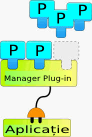
\includegraphics[]{PLA}
    \caption{Arhitectura Plug-in}
    \label{fig:imag35}
\end{figure}

\begin{center}
\rule{150mm}{.1pt}
\end{center}

\subsection{Interfața PLUG-IN-ului și descrierea \\ programatică a mecanismului de integrare dinamică}
